\chapter{Fotometria}

A fotometria é a ciência que mede a luz proveniente de um objeto, e quase toda informação que temos sobre o universo, vem na forma de luz. A luz  (ou partículas que compõem a luz, os fótons\footnote{Fóton é a unidade quântica elementar de luz. Na física quântica, os fótons são descritos como partículas discretas de energia que compõem a radiação eletromagnética e têm características tanto de onda quanto de partícula.}) é uma onda eletromagnética, vibrações elétricas e magnéticas, isto é, energia. As ondas eletromagnéticas são classificadas de acordo com seus comprimentos de onda e suas frequências, propriedades relacionadas às suas energias, quanto menor o comprimento de onda, maior a frequência e energia. Diferentes comprimentos de onda visíveis ao olho nu, chamamos de luz visível e relacionamos às cores, está, aproximadamente, no meio do espectro e abrange uma fração muito pequena, e todos os tipos de radiação juntos, denominamos de espectro eletromagnético.

\begin{figure}[h]
  \centering 
  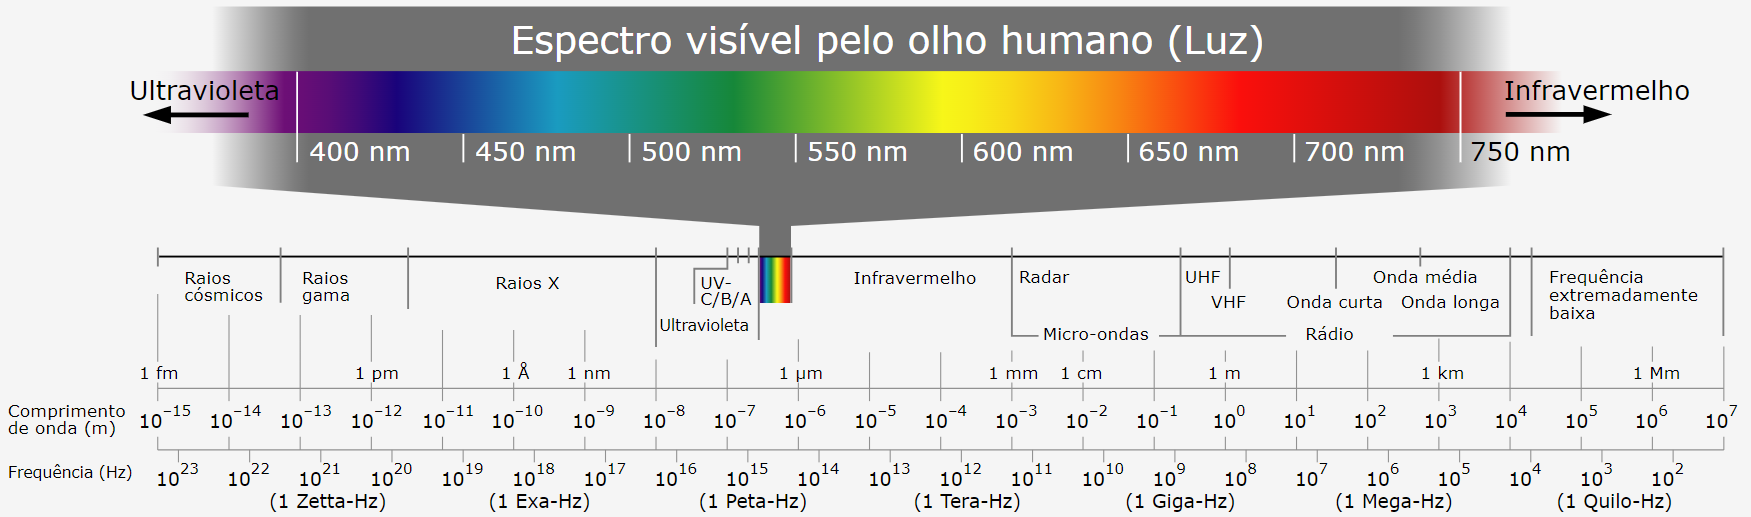
\includegraphics[width=1.0\textwidth]{Imagens/espectro.PNG} 
  \caption[Espectro eletromagnético.]{Espectro eletromagnético com todos os tipos de radiação eletromagnética que existem em nosso universo. Créditos: Horst Frank, Jailbird e Alebergen.}
  \label{fig:espectro} 
\end{figure}

Na astronomia, a fotometria teve início no final do século XIX e, nos últimos anos, diferentes tipos de detectores são utilizados para estudar a radiação electromagnética do universo, invisível aos nossos olhos. Há observações astronômicas que são feitas fora da atmosfera terrestre e na superfície da Terra. O espectro electromagnético, desde os raios gama até as ondas de rádio, são usados para observações astronômicas para estudar informações sobre a natureza e propriedades físico-químicas de uma fonte, como por exemplo, medir o fluxo e a cor de uma estrela e estimar sua temperatura. As câmeras digitais dos telescópios funcionam através do fenômeno físico denominado efeito fotoelétrico. Quando a luz (fóton) do objeto que estamos tirando ``foto'' atinge a lente (ou espelho) da câmera, esta lente focaliza a luz em um sensor de imagem, que é uma matriz de pequenos elementos fotoelétricos chamados de pixels. Cada pixel no sensor contém fotodetectores, que são sensíveis à luz, geralmente feitos de materiais semicondutores, como silício, chamados de CCD\footnote{Willard Boyle e George Smith criaram os CCDs em 1969 para uso como memória de computador. A primeira aplicação dos CCDs na astronomia como detectores ópticos ocorreu no final da década de 1970.} (do inglês, \emph{Charge Coupled Device}, dispositivo de carga acoplada). Quando a luz atinge os fotodetectores, ocorre o efeito fotoelétrico, liberando elétrons e gerando uma corrente elétrica proporcional à intensidade da luz. Os elétrons liberados pelo efeito fotoelétrico são coletados pelo pixel correspondente no sensor, quanto mais intensa for a luz incidente em um pixel, mais elétrons serão liberados e maior será a corrente elétrica gerada. Após a captura da luz pelos fotodetectores, os sinais elétricos gerados são convertidos em dados digitais, e cada pixel da imagem é representado por um valor numérico que indica a intensidade da luz capturada naquela área. Os dados digitais são processados pelo processador para melhorar a qualidade da imagem, remover ruídos, corrigir distorções e realizar análises científicas. Por fim, a imagem pode ser armazenada e visualizada. Quanto maior o número de pixels em um sensor CCD, maior área poderá ser capturada e representada na imagem final. Quanto menor o tamanho dos pixels, maior resolução da imagem, logo, mais pixels podem ser encaixados em uma determinada área do sensor. Todas as imagens astronômicas são feitas em preto e branco, em um gráfico de quantos fótons contribuíram com cada pixel, e coloridas majoritariamente, para que reflitam o que nossos olhos veriam se fossem sensíveis da mesma forma que os telescópios. Para isso, é necessário usar filtros, de forma que a luz de vários comprimentos de onda cheguem ao ponto focal do telescópio, mas somente os fótons permitidos pelos filtros são recebidos pelo detector.

\begin{figure}[h]
  \centering 
  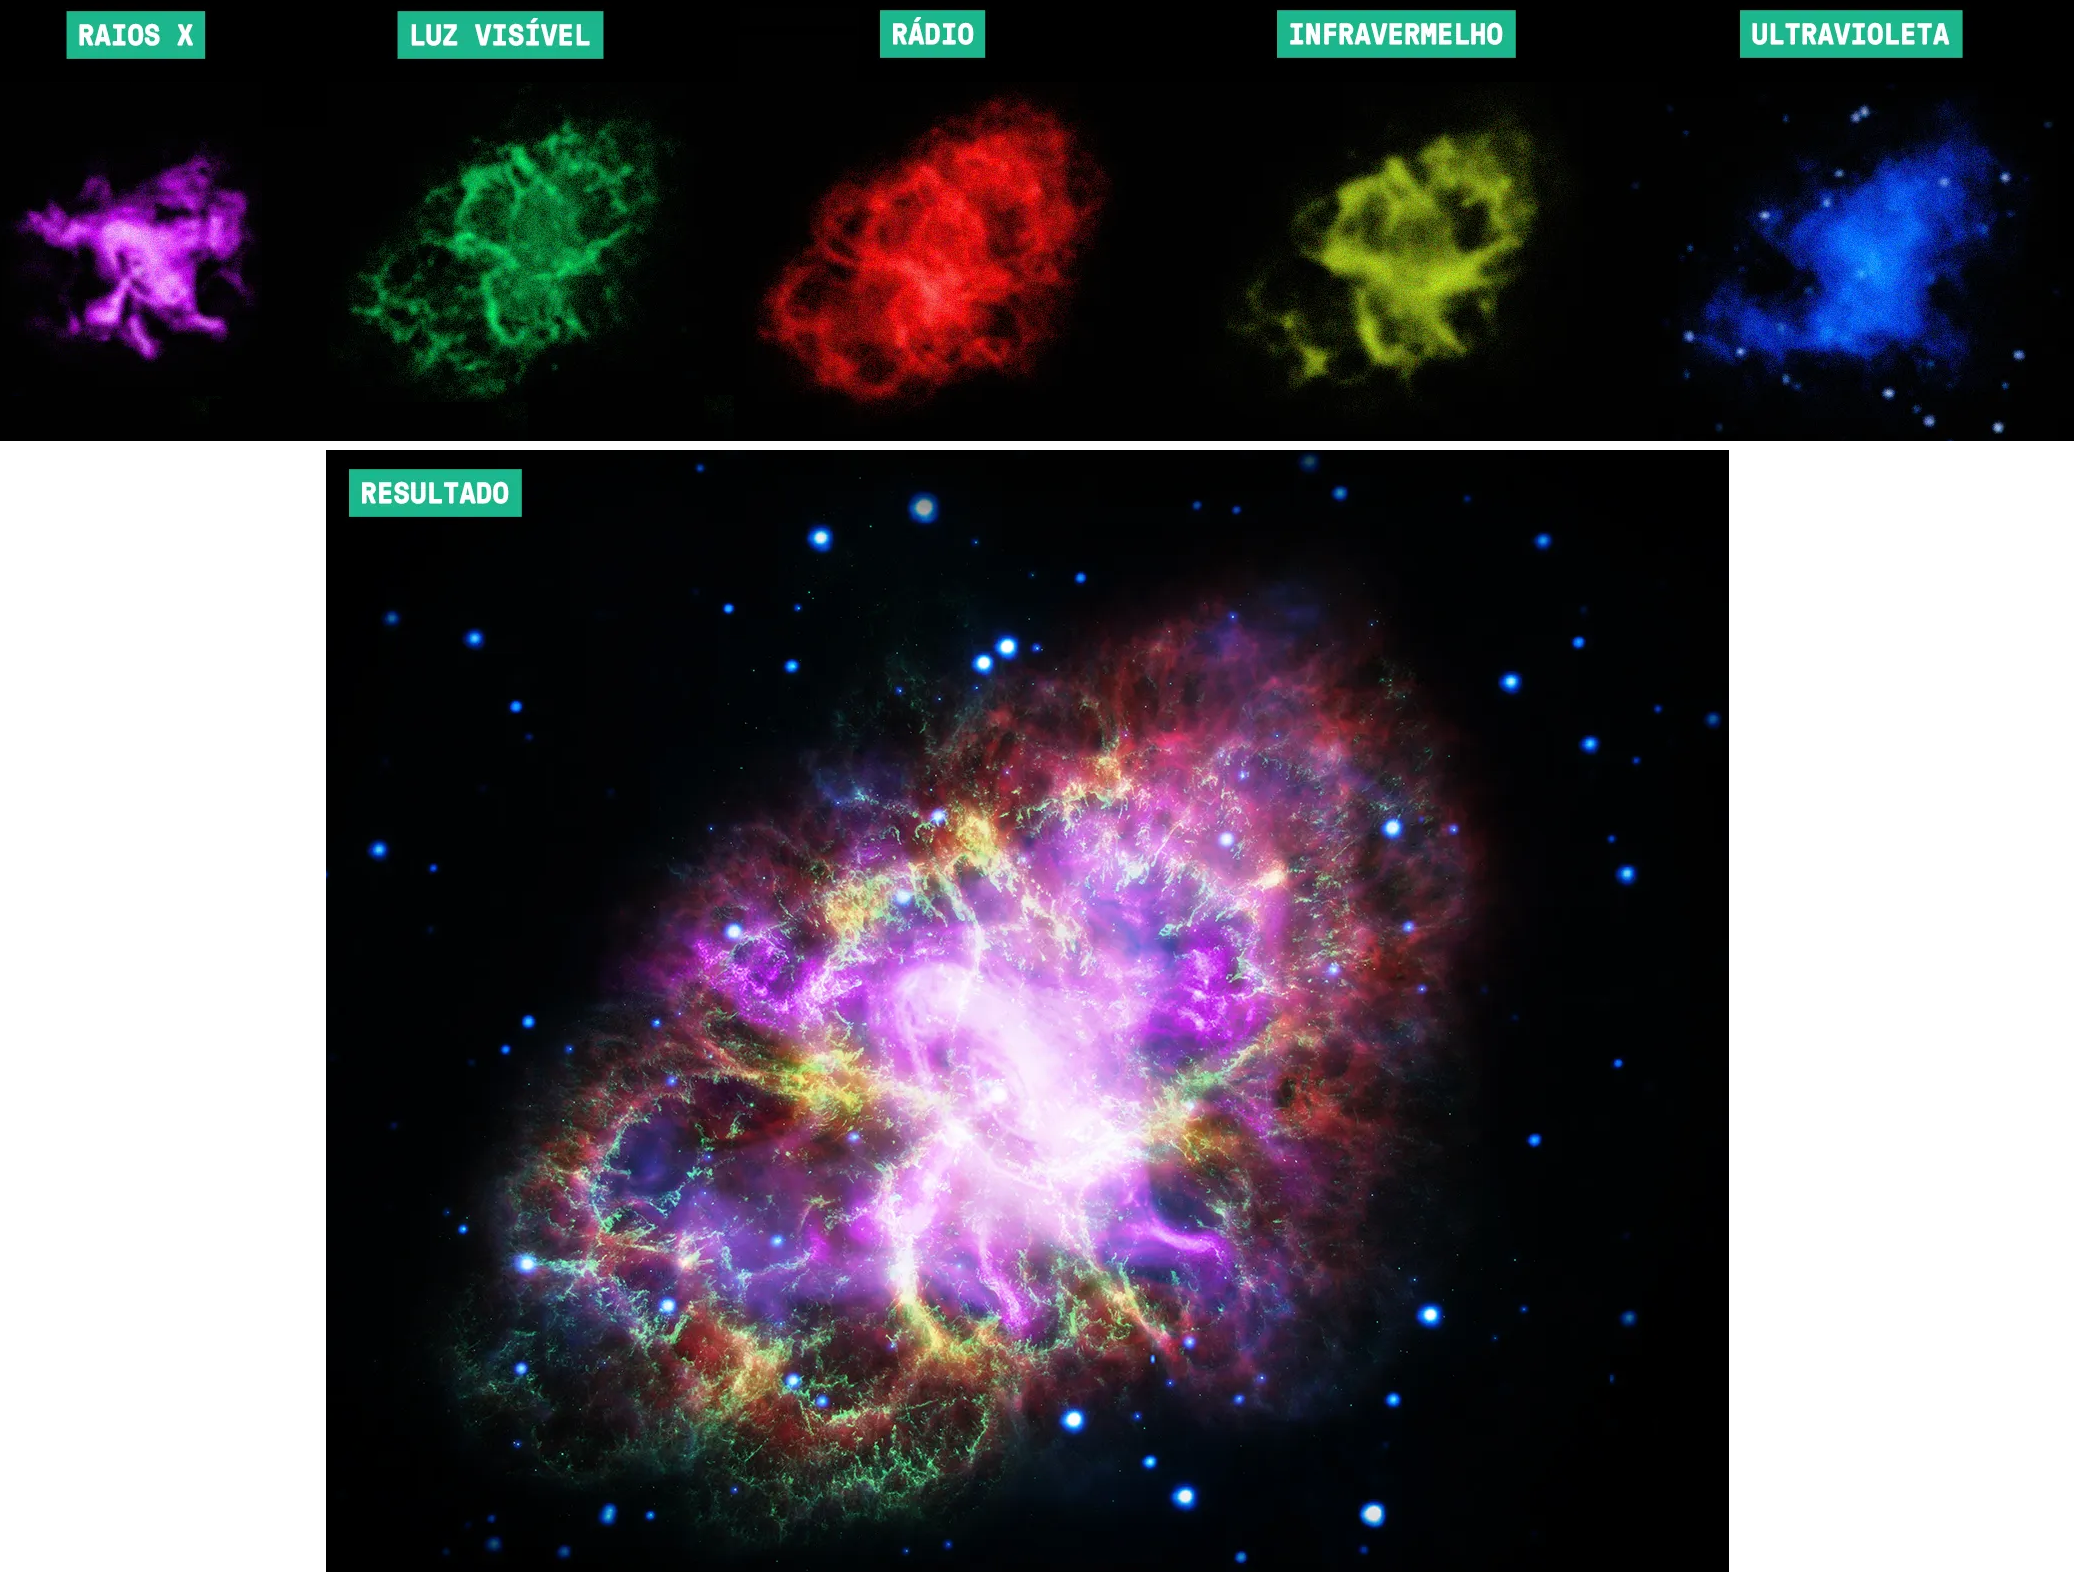
\includegraphics[width=0.77\textwidth]{Imagens/caranguejo_02.png} 
  \caption[Combinação de filtros para imagem da Nebulosa de Caranguejo.]{Combinação de filtros para imagem da Nebulosa de Caranguejo: raios-X, telescópio Chandra; luz visível, telescópio Hubble; ondas de rádio, observatório Very Large Array; infravermelho, telescópio Spitzer; ultravioleta, satélite X-ray Multi-Mirror-Newton. Créditos: NASA, ESA, G. Dubner et. al., NRAO e Caltech.}
  \label{fig:caranguejo} 
\end{figure}

A astronomia e astrofísica são ciências que dependem muito das observações, voltadas para imagens e processamento de imagens, portanto, os diferentes filtros representados por cores, em uma imagem combinada de filtros e cores, revelam, por exemplo, a composição química das nuvens de gás, poeira, estrelas e outros importantes componentes de uma galáxia. Para cada objeto astronômico precisa-se de métodos para a coloração das imagens geradas de acordo com seus filtros. Galáxias e nebulosas emitem mais luz em comprimentos de onda muito específicos devido aos componentes e elementos que as constituem, como o hidrogênio e oxigênio por exemplo. A quantidade de luz que recebemos de cada elemento traz informações importantes sobre a riqueza química e a física que está ocorrendo em um objeto astronômico, sendo essencial para a imagem o quanto dessa cor em específico existe. Para isso, é preciso cores para as bandas largas e bandas estreitas para os respectivos filtros. As bandas largas cobrem uma ampla região de comprimentos de onda. Por exemplo, uma banda larga pode cobrir uma grande faixa do espectro visível ou incluir uma parte significativa do infravermelho ou ultravioleta. As bandas estreitas, são faixas de comprimento de onda relativamente pequenas, e são selecionadas para observar características espectrais específicas, como linhas de emissão ou absorção de elementos químicos, regiões de alta ionização, ou outros fenômenos que são mais proeminentes em comprimentos de onda específicos. Para a atribuição de cores, cada projeto ou equipe adota uma lógica, por exemplo, como os raios-X são radiações energéticas, eles geralmente ficam com o violeta.

\begin{figure}[h]
  \centering 
  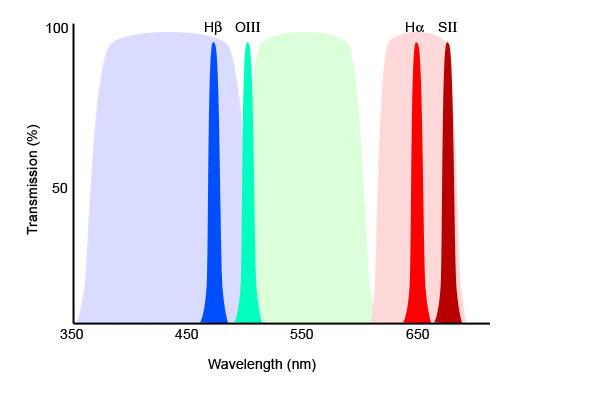
\includegraphics[width=0.8\textwidth]{Imagens/narrowbandandbroadband.jpg} 
  \caption[Exemplo de bandas estreitas combinadas com bandas largas.]{Exemplo de bandas estreitas (H\textbeta, OIII, H\textalpha\ e SII) combinadas com bandas largas (em azul, verde e vermelho claros). Créditos: tellescopio.com.br.}
  \label{fig:narrowbandandbroadband} 
\end{figure}

Para analisar as emissões de hidrogênio em uma nebulosa, por exemplo, o astrônomo pode usar filtro para a banda estreita centrada no comprimento de onda da emissão de hidrogênio para capturar especificamente esses sinais, isolando-os de outras fontes de luz e adotar a cor laranja para representá-lo. Para uma observação mais geral da nebulosa, pode ser usado um filtro de banda larga que abrange uma maior faixa de comprimentos de onda para obter uma visão mais ampla de suas características, como os filtros combinados (composição de imagens) ilustrados na Figura~\ref{fig:caranguejo}.

\section{Cor e temperatura}

Ao analisar a fotometria de uma galáxia, obtemos informações importantes sobre as estrelas que a compõe e suas características. Estrela é um corpo celeste massivo composto de gás, principalmente hidrogênio e hélio, mantido pela gravidade e capaz de gerar e emitir energia através de reações nucleares. As estrelas desempenham um papel fundamental na estrutura e na dinâmica das galáxias, podem ter diversos tamanhos, massa, temperatura, brilho e idades. Para entendermos alguns fenômenos que estão ocorrendo em uma galáxia e suas propriedades, precisamos conhecer suas estrelas. As estrelas apresentam um vasto domínio de cores, que refletem a temperatura em suas atmosferas em concordância com lei de Wien, que estabelece a relação entre a temperatura de pico da distribuição espectral de um corpo negro e sua temperatura absoluta. Um corpo negro é um objeto ideal que absorve toda a radiação incidente sobre ele e emite radiação térmica. As estrelas são excelentes modelos de corpos negros, ou "corpo negro equivalente", porque não refletem radiação, apenas emitem.

\afterpage{
\begin{figure}[h]
  \centering 
  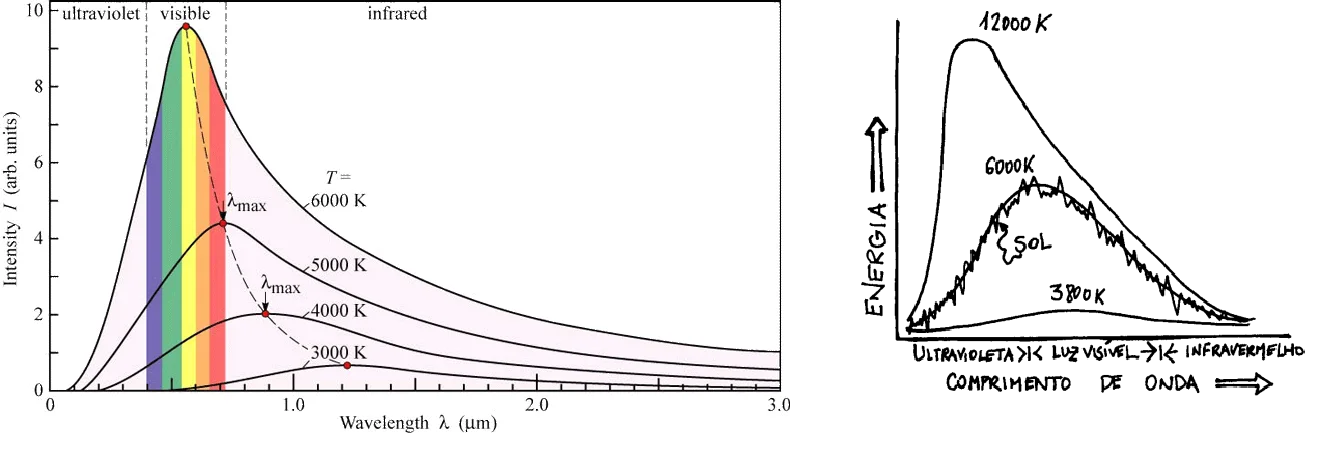
\includegraphics[width=1.0\textwidth]{Imagens/corponegro.png} 
  \caption[Distribuição espectral de um corpo negro.]{Esquerda\footnotemark[5]: curvas de distribuição espectral de um corpo negro. Direita\footnotemark[6]: quando comparamos a curva de distribuição de energia emitida do Sol com as curvas de distribuição de energia de um corpo negro, vemos seu pico da curva encontra-se no meio do espectro visível, próximo da cor verde-amarelo, aproximadamente 6 mil Kelvin (temperatura).}
  \label{fig:espectrosol}
\end{figure}
\footnotetext[5]{Fonte: https://cref.if.ufrgs.br/?contact-pergunta=radiacao-termica-e-ondas-eletromagneticas. Acesso em: 01 de maio de 2024.}
\footnotetext[6]{Fonte: https://fep.if.usp.br/~profis/arquivo/gref/optica17-2.pdf. Acesso em: 01 de maio de 2024.}
}

A cor de uma estrela é determinada pela parte de seu espectro visível que mais contribui para sua luminosidade total, que está intimamente ligada à sua temperatura superficial. Estrelas mais quentes têm espectros que atingem o pico em comprimentos de onda mais curtos, ou seja, mais azuis ou brancas, e as estrelas frias, mais vermelhas ou laranjas. Desta forma é possível conhecer a idade, composição química (especialmente a presença e a abundância de elementos como hidrogênio, hélio, metais e moléculas complexas), distribuição de massas em populações estelares e entender a evolução de uma região galáctica ou de uma galáxia como um todo ao longo do tempo. Ao estudar estrelas e suas cores, pode-se também identificar exoplanetas orbitando essas estrelas, encontrando zona habitável ao redor dela, onde a vida como a conhecemos poderia existir. Estrelas mais frias, como anãs vermelhas, têm zonas habitáveis mais próximas, enquanto estrelas mais quentes, como anãs brancas, têm zonas habitáveis mais distantes. A detecção de objetos de cores específicas, como supernovas\footnote[3]{Eventos astronômicos explosivos que marcam o fim da vida de certas estrelas, resultando em uma liberação extraordinária de energia.}, quasares\footnote[4]{Quasares, abreviação de "quasi-stellar radio source" (fonte de rádio quase estelar), são objetos astronômicos extremamente luminosos e distantes, considerados um tipo especial de núcleos ativos de galáxias (AGNs), regiões centrais de galáxias que emitem uma quantidade excepcional de energia em várias faixas do espectro eletromagnético.} e galáxias distantes, é essencial para mapear a distribuição espacial das galáxias e para estudar a expansão do universo.

\section{Magnitudes aparente e absoluta}

A magnitude aparente e a magnitude absoluta são fundamentais na astronomia para descrever o brilho de objetos. A magnitude aparente é uma medida do brilho (fluxo) percebido de um objeto a partir da Terra. É uma escala logarítmica inversa, o que significa que quanto menor o valor da magnitude aparente, mais brilhante é o objeto. Por exemplo, o Sol tem uma magnitude aparente de cerca de -26, enquanto uma estrela fraca visível a olho nu tem uma magnitude aparente de aproximadamente +6. Ao analisar um objeto, o fluxo obtido depende da sensibilidade espectral do equipamento utilizado para a observação, ou seja, do conjunto (telescópio + filtro + detector).

\[ \emph{m} = -2.5 \log_{10}(F) + c \]

Onde:

\emph{m} é a magnitude aparente do objeto;

\emph{F} é o brilho (fluxo de energia) medido do objeto (energia que chega ao detector);

\emph{c} é uma constante que depende da unidade de medida utilizada para B.

A magnitude absoluta é uma medida do brilho intrínseco de um objeto celeste e é definida como a magnitude que um objeto teria se estivesse a uma distância padrão de 10 parsecs (cerca de 32,6 anos-luz). A magnitude absoluta é útil para comparar o brilho real de objetos celestes sem ser influenciado pela sua distância.

\[ M = m - 5 \log_{10}(\frac{d}{10}) \]

Onde:

\emph{M}: representa a magnitude absoluta do objeto astronômico;

\emph{m}: representa a magnitude aparente do objeto astronômico.

\emph{d}: representa a distância do objeto em unidades astronômicas (UA).

Uma das formas de determinar a distância de um objeto astronômico, é usar a relação entre a luminosidade intrínseca (magnitude absoluta) e o brilho aparente. 

\section{Luminosidade}

A luminosidade de uma estrela é uma medida da quantidade total de energia que ela emite por unidade de tempo para o espaço ao seu redor. Essa energia pode ser emitida em várias faixas do espectro eletromagnético e está diretamente relacionada à sua temperatura efetiva, tamanho físico e taxa de emissão de energia. A luminosidade de uma estrela depende de seu tamanho e temperatura, se duas estrelas são do mesmo tamanho mas uma é mais quente que a outra, a mais quente será mais luminosa; se ambas têm a mesma temperatura, mas uma é maior que a outra, ela será mais luminosa.

Na astronomia, a luminosidade de uma estrela é geralmente medida em unidades solares (L\(_\odot\)), onde 1 unidade solar representa a luminosidade do Sol. Desta forma, uma estrela com uma luminosidade de 10 L\(_\odot\) emite dez vezes mais energia do que o Sol. Assim como estrelas individuais, a luminosidade de uma galáxia está relacionada à quantidade de estrelas que ela contém, à taxa de formação estelar, à presença de buracos negros supermassivos ativos, entre outros fatores. Galáxias podem ter uma ampla gama de luminosidades, desde galáxias anãs com baixa luminosidade até galáxias gigantes com luminosidades extremamente altas.

O diagrama Hertzsprung-Russell (HR), Figura~\ref{fig:diagramahr}, é uma ferramenta fundamental para representar e estudar os distintos estágios da evolução estelar. Ele foi desenvolvido por Ejnar Hertzsprung e Henry Norris Russell no início do século XX e é uma representação gráfica das luminosidades (ou magnitudes absolutas) das estrelas em relação às suas temperaturas efetivas (ou tipo espectral\footnote[7]{O sistema de classificação espectral, desenvolvido inicialmente por Annie Jump Cannon, divide as estrelas em sete classes designadas pelas letras O, B, A, F, G, K e M. Essas letras seguem uma sequência que reflete a temperatura efetiva das estrelas, onde as estrelas mais quentes são classificadas como tipo O e as mais frias como tipo M. Além das letras, as estrelas podem ser subdivididas numericamente de 0 a 9 dentro de cada classe principal. Por exemplo, uma estrela do tipo A0 é ligeiramente mais quente que uma estrela do tipo A1, enquanto uma estrela do tipo F5 é um pouco mais fria que uma estrela do tipo F6.}). As estrelas mais quentes (como as estrelas do tipo O e B) estão localizadas no lado esquerdo do diagrama, enquanto as estrelas mais frias (como as estrelas do tipo M) estão no lado direito. As estrelas mais luminosas estão localizadas na parte superior do diagrama, enquanto as estrelas menos luminosas estão na parte inferior. A sequência principal é uma faixa diagonal que representa a fase estável e principal da evolução estelar. Estrelas na sequência principal estão realizando fusão nuclear em seus núcleos, convertendo hidrogênio em hélio, fase que dura a maior parte da vida de uma estrela. 

\begin{figure}[h]
  \centering 
  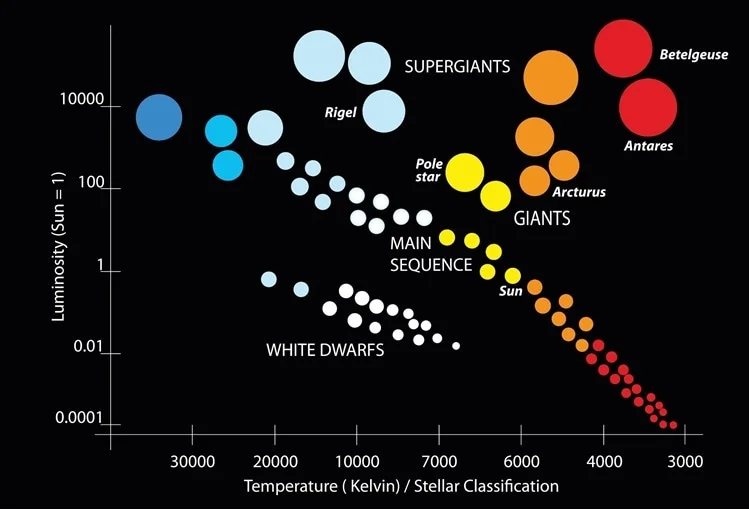
\includegraphics[width=0.8\textwidth]{Imagens/diagramahr.png} 
  \caption[Diagrama Hertzsprung-Russell.]{O eixo horizontal do diagrama HR representa a temperatura efetiva das estrelas, e o eixo vertical, a luminosidade, que está relacionada à quantidade de energia que uma estrela emite.}
  \label{fig:diagramahr} 
\end{figure}

As estrelas seguem caminhos específicos no diagrama HR à medida que evoluem ao longo de suas vidas, o que permite entender melhor os processos físicos que ocorrem nelas. Estrelas massivas comparadas às estrelas de pouca massa, envelhecem de formas diferentes e mudam de posições no diagrama; as massivas podem terminar suas vidas em explosões de supernova, deixando para trás remanescentes compactos como estrelas de nêutrons ou buracos negros, e as de pouca a média massa podem passar por estágios finais como anãs brancas, remanescentes compactos que esfriam ao longo do tempo.

\section{S-PLUS}

Os grandes levantamentos (\emph{surveys}), sejam eles espectroscópicos ou fotométricos, são muito importantes para nossa compreensão do universo. Esses levantamentos mapeiam a distribuição tridimensional de galáxias, aglomerados de galáxias e outras estruturas em largas escalas, de forma a ilustrar como o universo é organizado e como essas estruturas evoluíram ao longo do tempo. Ao examinar o espectro de luz de galáxias distantes, os \emph{surveys} espectroscópicos revelam informações valiosas sobre a história, evolução e expansão do universo, investigando a natureza da matéria escura e da energia escura, dois dos maiores desafios da física e da cosmologia modernas. Os levantamentos fotométricos fornecem informações detalhadas sobre a distribuição espacial, tamanho, forma, cor e luminosidade das galáxias. Isso é fundamental para investigar como as galáxias se formaram, evoluíram e se enriqueceram ao longo do tempo e como interagem umas com as outras em diferentes ambientes. A fotometria de alta precisão é essencial, por exemplo, na detecção e caracterização de exoplanetas (planetas fora do nosso sistema solar). Ambos os tipos de levantamentos desempenham um papel importante na astronomia, astrofísica e cosmologia, fornecendo dados para testar modelos teóricos e investigar fenômenos. 

Nesta pesquisa, trabalhamos com os dados fotométricos do Southern Photometric Local Universe Survey (S-PLUS) para estudar galáxias peculiares aneladas do hemisfério sul do universo local. O S-PLUS é um levantamento por imagem que cobrirá aproximadamente 8000 $\mathrm{graus}^{2}$ do céu do hemisfério sul em altas latitudes galácticas e cerca de 1300 $\mathrm{graus}^{2}$ sobre o disco e o bojo de nossa galáxia ao final do lançamento de seus dados, e utiliza um telescópio robótico (T80S) de abertura de 0,8 metros no Observatório Interamericano Cerro Tololo (CTIO), no Chile. Ele possui um sistema de 12 filtros, combinados em 5 bandas largas similares ao SDSS (Sloan Digital Sky Survey), $u$, $g$, $r$, $i$ e $z$, sendo que o filtro de banda $u$ é o filtro de \emph{Javalambre} e possui uma curva de transmissão mais eficiente comparada com a banda $u$ do SDSS, conforme descreve \citeonline{2019A&A...622A.176C}, e 7 bandas estreitas centradas em linhas de absorção e emissão específicas, importantes para caracterização da distribuição espectral de energias em classificação de estrelas, $[\text{OII}]$, Ca H+K, banda G, $H \delta$, tripleto de Mgb, $H \alpha$ e tripleto de Ca (ver \citeonline{2019MNRAS.489..241M}). O telescópio possui a câmera T80Cam-S e o detector (CCD) de matriz de 9232 × 9216 pixels, com uma escala de 0,55'' $\mathrm{pixel}^{-1}$ (segundos de arco por pixel) e um campo de visão (\emph{field of view}, FoV) de 1,4 × 1,4 graus.

\begin{figure}[h]
  \centering 
  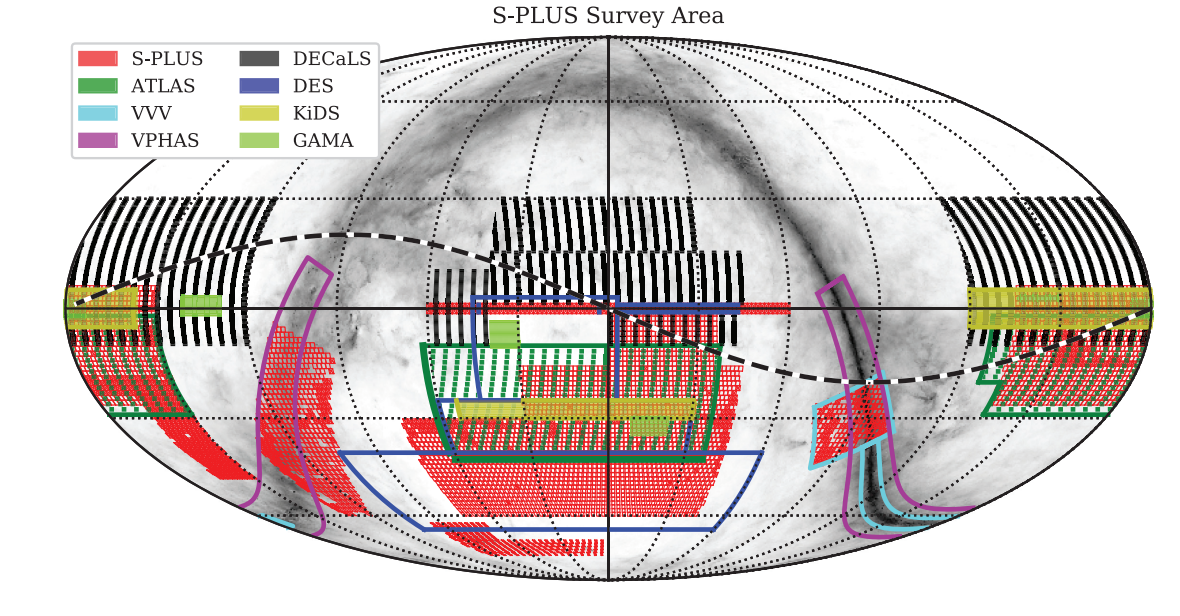
\includegraphics[width=0.9\textwidth]{Imagens/surveyarea.PNG} 
  \caption[Área de cobertura do S-PLUS.]{Em vermelho, a área de cobertura do S-PLUS, comparada a alguns levantamentos ópticos e de infravermelho próximo no hemisfério sul. Créditos: \citeonline{2019MNRAS.489..241M}.}
  \label{fig:surveyarea} 
\end{figure}

\begin{figure}[h]
  \centering 
  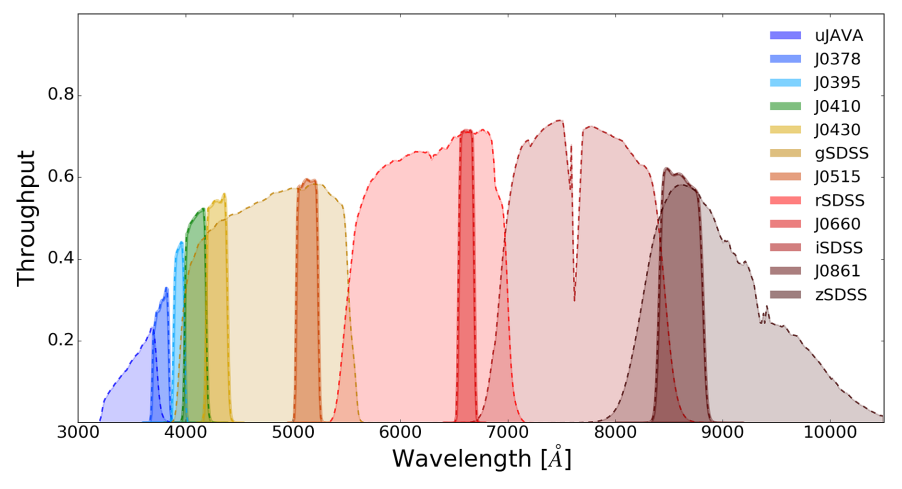
\includegraphics[width=0.8\textwidth]{Imagens/dozefiltros.PNG} 
  \caption[Sistema de 12 filtros do S-PLUS.]{A imagem mostra a eficiência total dos filtros em função do comprimento de onda. Diferentes cores são representadas para cada filtro de acordo com a legenda à direita. Os filtros J0378, J0395, J0410, J0430, J0515, J0660 e J0861 são, respectivamente, $[\text{OII}]$, Ca H+K, $H \delta$, banda G, tripleto de Mgb, $H \alpha$ e tripleto de Ca. Créditos: \citeonline{2019MNRAS.489..241M}.}
  \label{fig:dozefiltros} 
\end{figure}

\begin{figure}[h]
  \centering 
  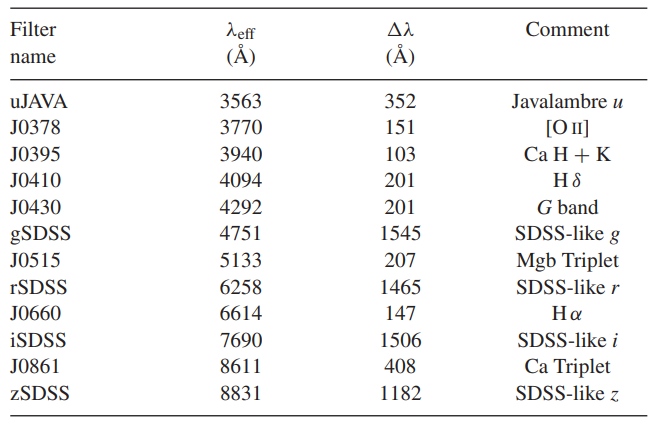
\includegraphics[width=0.7\textwidth]{Imagens/filtros.PNG} 
  \caption[Sumário dos filtros do S-PLUS.]{A tabela mostra as especificações dos comprimentos de onda centrais de cada filtro e a largura total à meia altura (FWHM\footnotemark[8]) das curvas de transmissão. Créditos: \citeonline{2019MNRAS.489..241M}.}
  \label{fig:filtros} 
\end{figure}
\footnotetext[8]{Do inglês, \emph{Full Width at Half Maximum} (Largura Total à Meia Altura), é uma medida de largura de um pico de distribuição que indica o intervalo entre os pontos em que a função tem metade do seu valor máximo.}

Uma das importantes vantagens do S-PLUS é o seu nível de resolução somado ao sistema de bandas estreitas para extrair informações de populações estelares, como idade e metalicidade, para uma grande quantidade de objetos. Ele fornecerá uma precisão de \emph{redshift} fotométrico z = 0.02 (ou melhor) para galáxias com r < 19.7 mag AB ou z < 0.4, e para galáxias com r < 21 mag AB ou z < 0.5, precisão de z = 0.03, grande mapeamento 3D do universo local (\citeonline{2019MNRAS.489..241M}; \citeonline{2022MNRAS.511.4590A}). O \emph{redshift} fotométrico é uma técnica utilizada na astronomia para estimar o desvio para o vermelho (z) de objetos astronômicos com base em suas características espectrais capturadas em imagens fotométricas, uma maneira rápida e eficiente (em termos de tempo de observação) de estimar \emph{redshift}\footnote[9]{O redshift descreve o deslocamento das linhas espectrais de um objeto em direção ao espectro do vermelho. Esse desvio para o vermelho é uma medida do quão longe e quão rápido um objeto se afasta de nós no espaço (ou blueshift, deslocamento das linhas espectrais de um objeto em direção ao espectro do azul, e ocorre quando o objeto está se aproximando do observador), bem como à expansão do Universo.} para um grande número de objetos, e com isso, estudar a velocidade, direção do movimento e distribuição espacial de galáxias, evolução do universo, determinar distâncias e outras ciências. 

Os dados do catálogo fotométrico multi-banda incluem as magnitudes medidas em seis aberturas diferentes para cada filtro. As aberturas são geradas executando o software SExtractor\footnote[10]{Documentação: https://sextractor.readthedocs.io/en/latest/index.html.} \cite{1996A&AS..117..393B}: aberturas elípticas variáveis (auto e petro), abertura isofotal (iso), aberturas aper 3 e aper 6 circulares fixas e a abertura circular PStotal. O SExtractor, inicialmente, realiza a análise completa de uma imagem de forma totalmente automatizada. Para detectar objetos mais fracos, por exemplo, e fazer medições precisas, o software calcula uma estimativa do nível de fundo em qualquer posição da imagem: um mapa de fundo. O modelo do fundo do céu é construído e computadas as estatísticas. Os pixels da imagem são subtraídos desse fundo e filtrados. As detecções são então limpas e medidas. Por fim, as quantidades medidas são escritas no catálogo de saída. As medições são feitas nos contornos isofotais dos objetos, definidos na imagem de detecção filtrada. Somente pixels com valores acima do limiar de detecção (fundo) são considerados e constituem o contorno isofotal. Uma vez encontrados estes pixels, o algoritmo do software opera parâmetros (denominados de \emph{primeiro momento}) para as aberturas elípticas: as coordenadas do baricentro (x e y), para definir a posição do ``centro'' de uma fonte; formatos básicos elípticos (eixo maior A, eixo menor B e ângulo de inclinação Theta) para representar a dispersão espacial máxima e mínima do perfil do objeto ao longo de qualquer direção; e elongação e elipticidade (parâmetros de elipse derivados de A e B). As magnitudes das aberturas estão expressas no sistema AB (Absolute AB) e todos os valores dos parâmetros para cada fonte detectada são fornecidos pelo S-PLUS. Nesta pesquisa, trabalhamos com as aberturas elípticas variáveis auto, petro e a abertura isofotal para o estudo de galáxias peculiares aneladas.

\begin{figure}[h]
  \centering 
  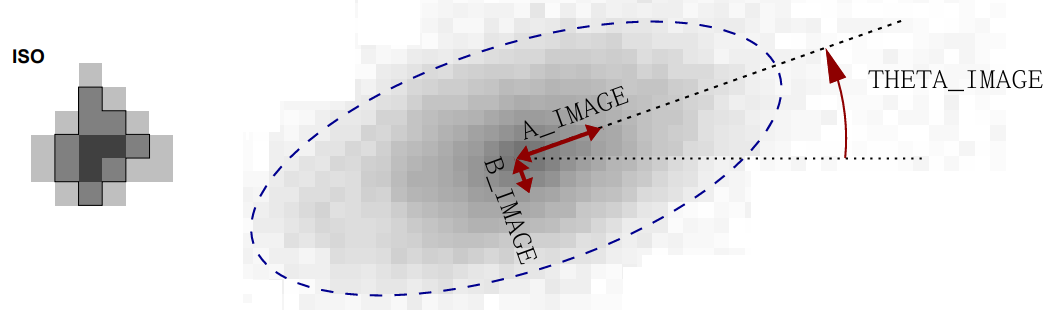
\includegraphics[width=0.7\textwidth]{Imagens/iso_elipse.png} 
  \caption[Detecção de uma fonte e parâmetros da elipse.]{Exemplo de uma detecção de pixels com valores acima do limiar (iso) e os parâmetros de formatos básicos de uma elipse computados em seguida.}
  \label{fig:iso_elipse} 
\end{figure}

\subsection{Abertura ISO}
Iso: A partir das medições do \emph{primeiro momento} (x, y, A, B, theta, elongação e elipticidade) feitas nos contornos isofotais das detecções, um parâmetro escalar (denominado \emph{segundo momento}, equação \ref{eq:parametro_escalar}), é computado para dimensionar a elipse, denominado de R, baseado em CXX, CYY e CXY (baricentros que também representam a mesma elipse). Desta forma, a área isofotal total é obtida para cada fonte.
\newcommand{\CXX}{C_{\text{XX}}}
\newcommand{\CYY}{C_{\text{YY}}}
\newcommand{\CXY}{C_{\text{XY}}}
\begin{equation} \label{eq:parametro_escalar}
\CXX(x-\bar{x})^2 + \CYY(y-\bar{y})^2 + \CXY(x-\bar{x})(y-\bar{y}) = R^2
\end{equation}

Geralmente, o limite isofotal de um objeto detectado é bem representado por $R \approx 3$, mas para fontes estendidas esse parâmetro varia. O fluxo ISO para cada filtro é determinado pela equação \ref{eq:fluxo_iso}, onde \emph{pi} são os pixels detectados acima do fundo e \emph{S} a distribuição espacial dos pixels:
\begin{equation} \label{eq:fluxo_iso}
\displaystyle
\sum_{i \in S} pi
\end{equation}

\begin{figure}[h]
  \centering 
  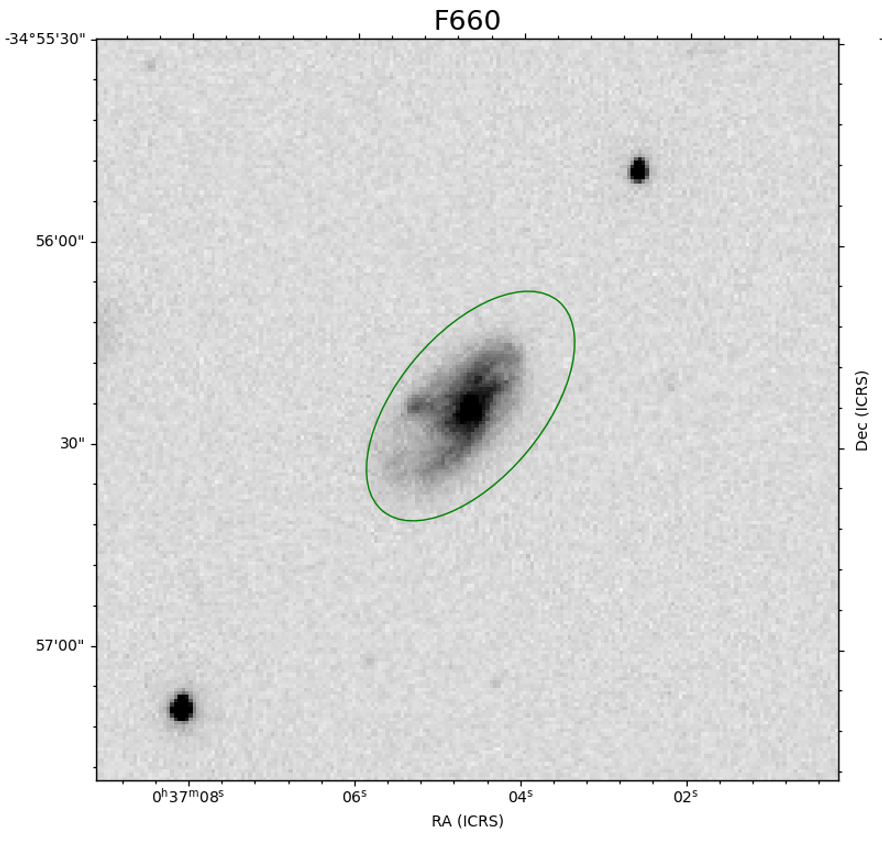
\includegraphics[width=0.6\textwidth]{Imagens/iso_exemplo.png} 
  \caption[Exemplo da abertura ISO para a galáxia AM 0034-351.]{Exemplo da abertura ISO computada usando o SExtractor pelo S-PLUS para a galáxia peculiar anelada AM 0034-351.}
  \label{fig:iso_exemplo} 
\end{figure}

\subsection{Abertura elíptica variável AUTO}
Auto: Definida em termos do raio de \citeonline{1980ApJS...43..305K} e obtida a partir das medições do \emph{primeiro momento} (x, y, A, B, theta, elongação e elipticidade) feitas nos contornos isofotais das detecções. Os eixos A e B da elipse são multiplicados por 6 (o que corresponde aproximadamente a duas vezes o tamanho do contorno isofotal em cada eixo). O fator de Kron (raio de Kron) é calculado dentro dessa abertura elíptica pela equação \ref{eq:kron_radius} e a elipse de Kron (abertura auto) determinada, onde \emph{pi} são os pixels na imagem de detecção acima do fundo, \emph{ri} é o ``pseudo-raio reduzido'' no pixel \emph{i} e \emph{E} a abertura elíptica.
\begin{equation} \label{eq:kron_radius}
\scalebox{1.2}{$\displaystyle \frac{\sum_{i \in \mathit{E}} ri \, pi}{\sum_{i \in \mathit{E}} pi}$}
\end{equation}

A abertura elíptica de Kron (abertura auto) é a elipse com o raio de Kron aplicado ao \emph{primeiro momento} do algoritmo. Objetos com muito ruído podem acabar com uma elipse de Kron pequena, desta forma, o SExtractor impõe um tamanho mínimo para o raio de Kron para 2.0 e máximo de 3.5. O S-PLUS alterou os parâmetros para 1.82 e 3.00 para melhor representar a magnitude total das fontes. Após a abertura elíptica auto gerada, o fluxo das fontes para cada filtro é calculado pela soma dos valores dos pixels em unidas de AB mag pela equação \ref{eq:kron_flux}, onde \emph{K} é a abertura elíptica de Kron.
\begin{equation} \label{eq:kron_flux}
\displaystyle
\sum_{i \in K} pi
\end{equation}

\begin{figure}[h]
  \centering 
  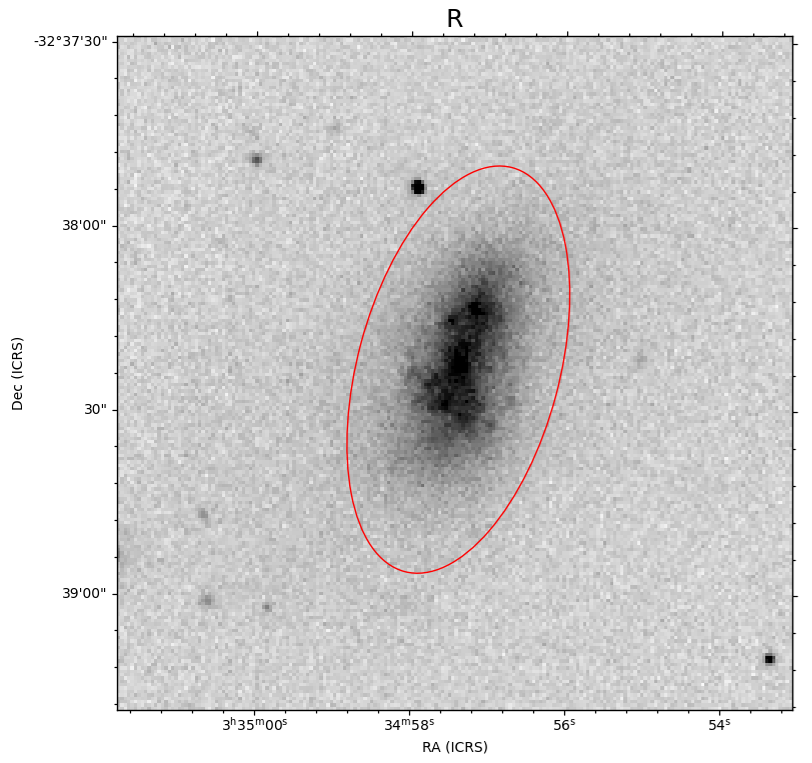
\includegraphics[width=0.6\textwidth]{Imagens/auto_exemplo.png} 
  \caption[Exemplo da abertura AUTO para a galáxia AM 0332-324.]{Exemplo da abertura AUTO em termos do raio de Kron computada usando o SExtractor pelo S-PLUS para a galáxia peculiar anelada AM 0332-324.}
  \label{fig:auto_exemplo} 
\end{figure}

\subsection{Abertura elíptica variável PETRO}
Petro: Similar à abertura auto, a abertura elíptica variável petro é definida em termos do raio de Petrosian\cite{1976ApJ...209L...1P}. Uma vez obtida as medições do \emph{primeiro momento} (x, y, A, B, theta, elongação e elipticidade) feitas nos contornos isofotais das detecções, os eixos A e B da elipse também são multiplicados por 6 e o fator de Petrosian (raio de Petrosian) é calculado dentro dessa abertura elíptica pela equação \ref{eq:petro_radius} e a elipse de Petro (abertura petro) determinada, onde \emph{pi} são os pixels na imagem de detecção acima do fundo e \emph{ri} é o ``pseudo-raio reduzido'' no pixel \emph{i}.
\begin{equation} \label{eq:petro_radius}
\scalebox{1.2}{$\displaystyle \left(\frac{\sum_{0.9r<ri<1.1r} p_i}{\sum_{ri<r} p_i}\right) \cdot \left(\frac{N_{\underset{ri<r}{\ }}}{N_{\underset{0.9r<ri<1.1r}{\ }}}\right)$}
\end{equation}

A abertura elíptica de Petrosian (abertura petro) é a elipse com o raio de Petrosian aplicado ao \emph{primeiro momento} do algoritmo. Da mesma forma que a abertura auto, o SExtractor impõe um tamanho mínimo para o raio de Petrosian para 2.0 e máximo de 3.5. O S-PLUS alterou os parâmetros para 2.0 e 2.73, respectivamente. Após a abertura elíptica petro gerada, o fluxo das fontes para cada filtro é calculado pela soma dos valores dos pixels, em unidas de AB mag, pela equação \ref{eq:petro_flux}, onde \emph{P} é a abertura elíptica de Petrosian e \emph{pi} são os pixels detectados acima do fundo. 
\begin{equation} \label{eq:petro_flux}
\displaystyle
\sum_{i \in P} pi
\end{equation}

\begin{figure}[h]
  \centering 
  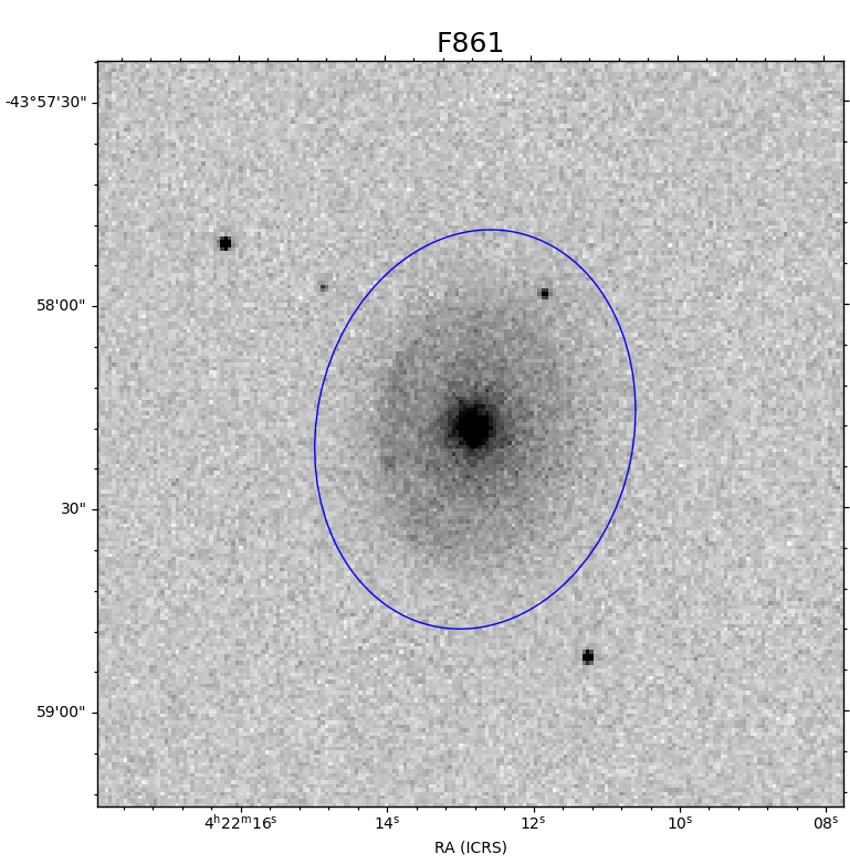
\includegraphics[width=0.6\textwidth]{Imagens/petro_exemplo.PNG} 
  \caption[Exemplo da abertura PETRO para a galáxia AM 0420-440.]{Exemplo da abertura PETRO em termos do raio de Petrosian computada usando o SExtractor pelo S-PLUS para a galáxia peculiar anelada AM 0420-440.}
  \label{fig:petro_exemplo} 
\end{figure}

Todos os parâmetros computados possuem seus respectivos erros estimados e são fornecidos pelo S-PLUS para cada filtro e abertura. O S/N\footnote[11]{A relação sinal-ruído (S/N) avalia a confiabilidade e a precisão das medições de fluxo luminoso ou de intensidade de um objeto em relação ao ruído de fundo associado a ele.} é definido como o fluxo dividido pelo seu erro e para a não detecção em um determinado filtro, a magnitude é substituída por 99.


